\documentclass[tikz,border=3pt]{standalone}
\usepackage[T1]{fontenc}
\usepackage[utf8]{inputenc}
\usepackage[english]{babel}
\usepackage{mathptmx}
\usepackage[scaled=0.92]{helvet}
\usepackage{amsmath,amssymb,textcomp}
\usetikzlibrary{positioning,arrows.meta}
\newcommand{\us}{\textmu s}
\begin{document}
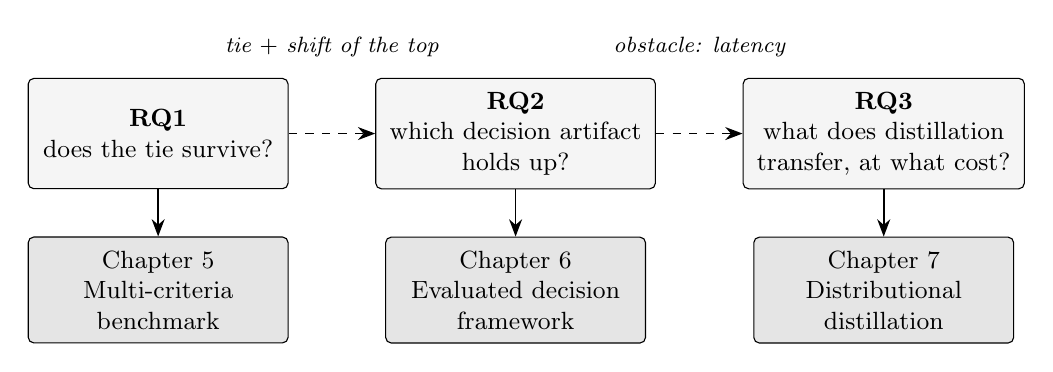
\begin{tikzpicture}[
  font=\small,
  qp/.style={draw, rounded corners=2pt, align=center, inner sep=5pt,
             minimum width=33mm, minimum height=14mm, fill=black!4},
  capbox/.style={draw, rounded corners=2pt, align=center, inner sep=5pt,
              minimum width=33mm, minimum height=12mm, fill=black!10},
  lig/.style={-{Stealth[length=2.2mm]}, semithick},
  enc/.style={-{Stealth[length=2.2mm]}, semithick, dashed},
  rot/.style={font=\footnotesize\itshape, midway, above=8.5mm},
  node distance=6mm and 11mm]

\node[qp] (qp1) {\textbf{RQ1}\\does the tie survive?};
\node[qp, right=of qp1] (qp2) {\textbf{RQ2}\\which decision artifact\\holds up?};
\node[qp, right=of qp2] (qp3) {\textbf{RQ3}\\what does distillation\\transfer, at what cost?};

\node[capbox, below=of qp1] (c5) {Chapter~5\\Multi-criteria\\benchmark};
\node[capbox, below=of qp2] (c6) {Chapter~6\\Evaluated decision\\framework};
\node[capbox, below=of qp3] (c7) {Chapter~7\\Distributional\\distillation};

\draw[lig] (qp1) -- (c5);
\draw[lig] (qp2) -- (c6);
\draw[lig] (qp3) -- (c7);
\draw[enc] (qp1.east) -- node[rot] {tie $+$ shift of the top} (qp2.west);
\draw[enc] (qp2.east) -- node[rot] {obstacle: latency} (qp3.west);
\end{tikzpicture}
\end{document}
